%% ============================================================
%%  MANUAL DE USO — Línea de Costa (cv-lit)
%%  Documento independiente: SOLO cómo usar la aplicación instalada.
%%  Para la memoria técnica completa (arquitectura, algoritmos, historial),
%%  ver memoria.tex / memoria.pdf en esta misma carpeta.
%% ============================================================
\documentclass[12pt,a4paper,spanish]{article}

% -- Codificación y tipografía --------------------------------
\usepackage[T1]{fontenc}
\usepackage[utf8]{inputenc}
\DeclareUnicodeCharacter{25CF}{\ensuremath{\bullet}}
\DeclareUnicodeCharacter{25B6}{\ensuremath{\triangleright}}
\DeclareUnicodeCharacter{25A0}{\ensuremath{\blacksquare}}
\DeclareUnicodeCharacter{2713}{\ensuremath{\checkmark}}
\usepackage[spanish,es-noquoting]{babel}
\usepackage{lmodern}
\usepackage{microtype}

% -- Geometría ------------------------------------------------
\usepackage[
  top=2.5cm, bottom=2.5cm,
  left=3.0cm, right=2.5cm,
  headheight=15pt
]{geometry}

% -- Color y gráficos -----------------------------------------
\usepackage[dvipsnames,svgnames,table]{xcolor}
\usepackage{graphicx}
\usepackage{float}

% -- Tablas ---------------------------------------------------
\usepackage{booktabs}
\usepackage{array}
\newcolumntype{L}[1]{>{\raggedright\arraybackslash}p{#1}}
\newcolumntype{C}[1]{>{\centering\arraybackslash}p{#1}}

% -- Código fuente (solo texttt inline, este manual no lleva bloques minted) --
\usepackage{enumitem}
\usepackage{parskip}
\setlength{\parskip}{6pt}

% -- Cabeceras y pies -------------------------------------------
\usepackage{fancyhdr}
\pagestyle{fancy}
\fancyhf{}
\fancyhead[L]{\small\textit{Línea de Costa --- Manual de Uso}}
\fancyhead[R]{\small\textit{\leftmark}}
\fancyfoot[C]{\thepage}
\renewcommand{\headrulewidth}{0.4pt}

% -- Hiperenlaces ---------------------------------------------
\usepackage[
  colorlinks=true,
  linkcolor=NavyBlue,
  urlcolor=Teal,
  pdftitle={Línea de Costa --- Manual de Uso},
  pdfauthor={Tech4D Lab --- Universidad de Alicante}
]{hyperref}

% -- Cajas de información -------------------------------------
\usepackage{tcolorbox}
\tcbuselibrary{skins,breakable}
\newtcolorbox{infobox}[1][]{
  colback=SkyBlue!10, colframe=NavyBlue!70,
  fonttitle=\bfseries, title=#1,
  breakable, left=6pt, right=6pt, top=4pt, bottom=4pt
}
\newtcolorbox{warnbox}[1][]{
  colback=Goldenrod!12, colframe=Goldenrod!80,
  fonttitle=\bfseries, title=#1,
  breakable, left=6pt, right=6pt, top=4pt, bottom=4pt
}

% -- Títulos ----------------------------------------------------
\usepackage{titlesec}
\titleformat{\section}
  {\normalfont\Large\bfseries\color{NavyBlue!80}}
  {\thesection}{1em}{}
\titleformat{\subsection}
  {\normalfont\large\bfseries\color{NavyBlue!60}}
  {\thesubsection}{1em}{}

% -- Metadatos ------------------------------------------------
\title{%
  \vspace{-1.5cm}
  \textbf{\Huge Manual de Uso}\\[0.4cm]
  {\Large\textcolor{NavyBlue}{Línea de Costa}}\\[0.2cm]
  {\large Sistema de Monitorización Automática de Línea de Costa}\\[0.6cm]
  \rule{\linewidth}{1pt}\\[0.4cm]
  {\normalsize Guardamar del Segura · Alicante · España}
}
\author{Tech4D Lab --- Universidad de Alicante}
\date{Septiembre 2026}

%% ============================================================
\begin{document}
%% ============================================================

\maketitle
\thispagestyle{empty}

\begin{abstract}
\noindent
Este documento explica \textbf{únicamente cómo usar} la aplicación de escritorio
\textbf{Línea de Costa} ya instalada — pantalla por pantalla, con capturas reales. No cubre
arquitectura, algoritmos ni código: para eso está la memoria técnica completa del proyecto
(\texttt{memoria.pdf}).
\end{abstract}

\tableofcontents

% ==============================================================

\section{Abrir la aplicación}

Para el uso normal no hace falta Python, Node.js ni ninguna terminal: se instala el ejecutable
de Windows y se abre como cualquier otro programa.

\begin{enumerate}[leftmargin=1.5em]
  \item Ejecutar \texttt{LineaDeCosta-Setup.exe} y seguir el asistente de instalación.
  \item Abrir \textbf{``Línea de Costa''} desde el menú Inicio o el acceso directo del
        escritorio.
  \item La primera vez puede tardar unos segundos en aparecer la ventana: el propio ejecutable
        arranca primero el backend en segundo plano y luego abre la ventana nativa apuntando a
        él — no hace falta ningún navegador aparte.
\end{enumerate}

\begin{warnbox}[No usar el acceso directo ``Descargar modelo de IA (SAM)'' para el uso normal]
El instalador crea, además del acceso a la app, uno secundario en el menú Inicio para
\emph{forzar} la descarga del checkpoint de SAM ($\sim$2,4~GB) sin abrir la ventana — solo hace
falta si SAM no se instaló bien la primera vez o se quiere volver a descargar aposta. Abrirlo por
error solo muestra una consola que imprime una línea y se cierra sola; no es un fallo, pero
confunde si se pulsa pensando que es la app.
\end{warnbox}

\begin{warnbox}[Transectos y Entrenamiento: ocultos del menú a día de hoy (23/09/2026)]
A petición del usuario, las pantallas \textit{Transectos} (\S\ref{sec:transectos}) y
\textit{Entrenamiento (temp.)} (\S\ref{sec:entrenamiento}) \textbf{no tienen botón de acceso en
el menú lateral} en esta versión — se ocultaron, no se eliminaron: siguen intactas y
funcionando por dentro (un transecto ya marcado, por ejemplo, se sigue calculando en cada
análisis). Este manual las documenta igualmente porque pueden reactivarse en cualquier momento.
Las capturas de este manual corresponden a la interfaz \textbf{tal y como se ve ahora mismo},
sin esos dos botones.
\end{warnbox}

\section{Recorrido por pantallas}

El menú lateral agrupa las pantallas en dos bloques: \textbf{Proceso} (el trabajo diario) y
\textbf{Sistema} (configuración y mantenimiento, se toca con menos frecuencia).

\subsection{Dashboard}

Vista general: estado de calibración de las 6 cámaras, gráfica de evolución histórica del área
seca y accesos rápidos a cada cámara.

\begin{figure}[H]
\centering
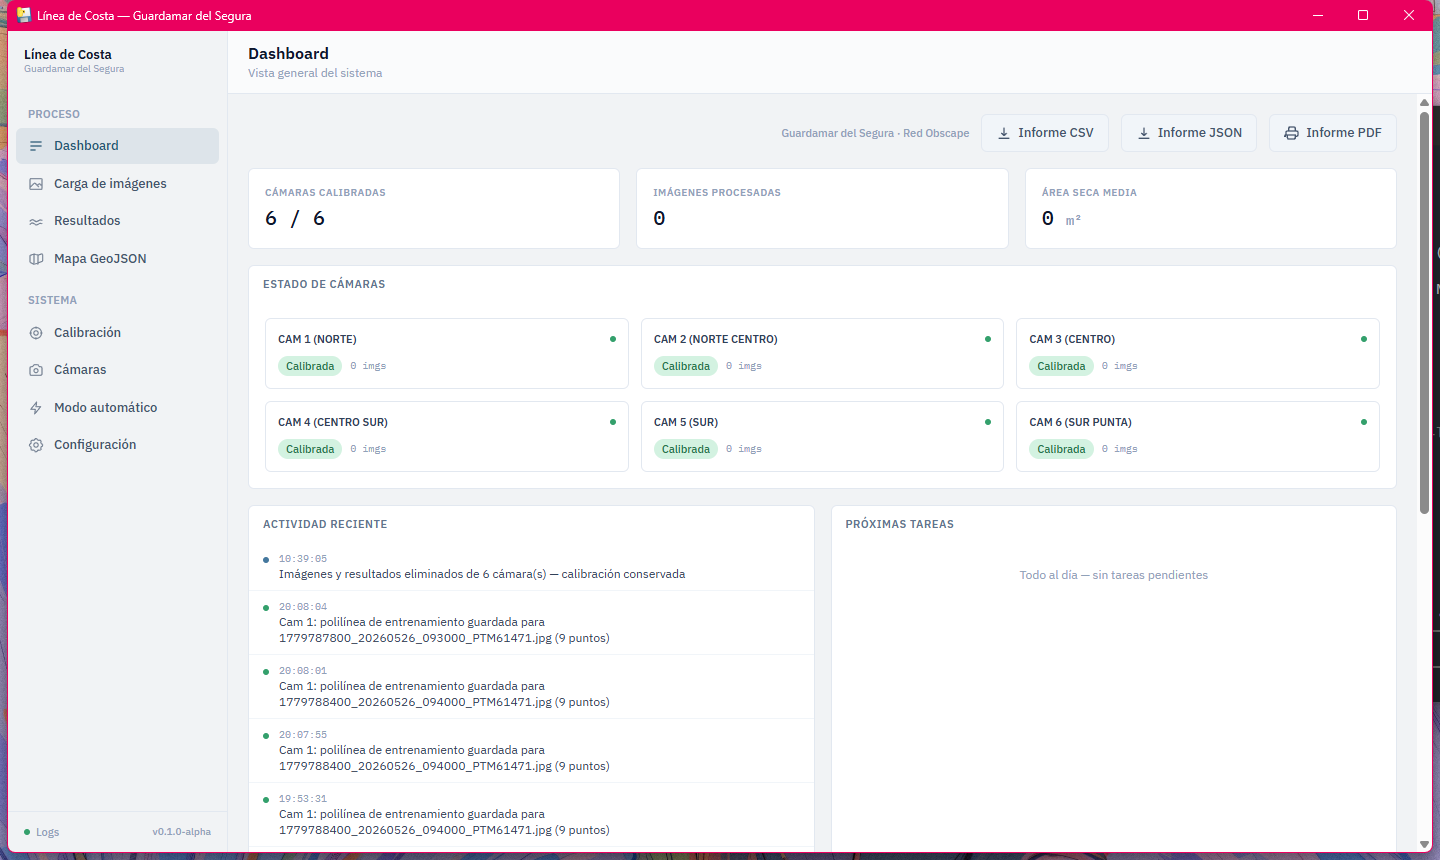
\includegraphics[width=0.95\textwidth]{screenshots/01_dashboard.png}
\caption{Dashboard, con las 6 cámaras calibradas y el botón \textit{Informe PDF}.}
\end{figure}

\subsection{Carga de imágenes}

Pantalla para gestionar qué imágenes tiene cada cámara y lanzar su análisis.

\begin{itemize}[leftmargin=1.5em]
  \item \textbf{Subir imágenes}: arrastrar archivos a la zona punteada, o hacer clic para elegir
        con el explorador.
  \item \textbf{Filtro de fechas}: acota la cuadrícula de miniaturas a un rango \emph{desde/hasta}.
  \item \textbf{Selección}: clic sobre una miniatura para marcarla/desmarcarla; \textit{Todas} /
        \textit{Ninguna} / \textit{Solo H:00h} (la hora con más fotos del filtro actual) la
        rellenan de golpe.
  \item \textbf{Previsualizar antes de procesar}: el icono de lupa que aparece al pasar el ratón
        sobre una miniatura abre la foto real a tamaño completo — la miniatura es demasiado
        pequeña para juzgar si una imagen sirve (niebla, cámara movida, algo tapando la zona).
        Desde ese mismo visor se puede \textbf{Descartar} (elimina el archivo) o \textbf{Cerrar}
        sin tocar nada.
  \item \textbf{Punto verde} en una miniatura: esa imagen ya tiene un resultado aceptado en el
        histórico.
  \item \textbf{Botón de la papelera} (esquina inferior derecha de la miniatura, aparece al
        pasar el ratón): borra la imagen directamente, con confirmación.
  \item \textbf{Botones de proceso}, de izquierda a derecha:
    \begin{itemize}
      \item \textit{Reanalizar todas (N)} — repite el análisis de TODAS las imágenes del filtro
            actual, incluidas las ya analizadas. Hace falta tras una mejora de la segmentación,
            para refrescar resultados antiguos.
      \item \textit{Analizar pendientes (N)} — solo las que nunca se han analizado.
      \item \textit{Procesar selección (N)} — solo las marcadas a mano.
    \end{itemize}
        Las tres procesan las imágenes \textbf{una a una} (no se puede en lote) y al terminar
        llevan a \textit{Resultados} con la última imagen procesada.
\end{itemize}

\begin{figure}[H]
\centering
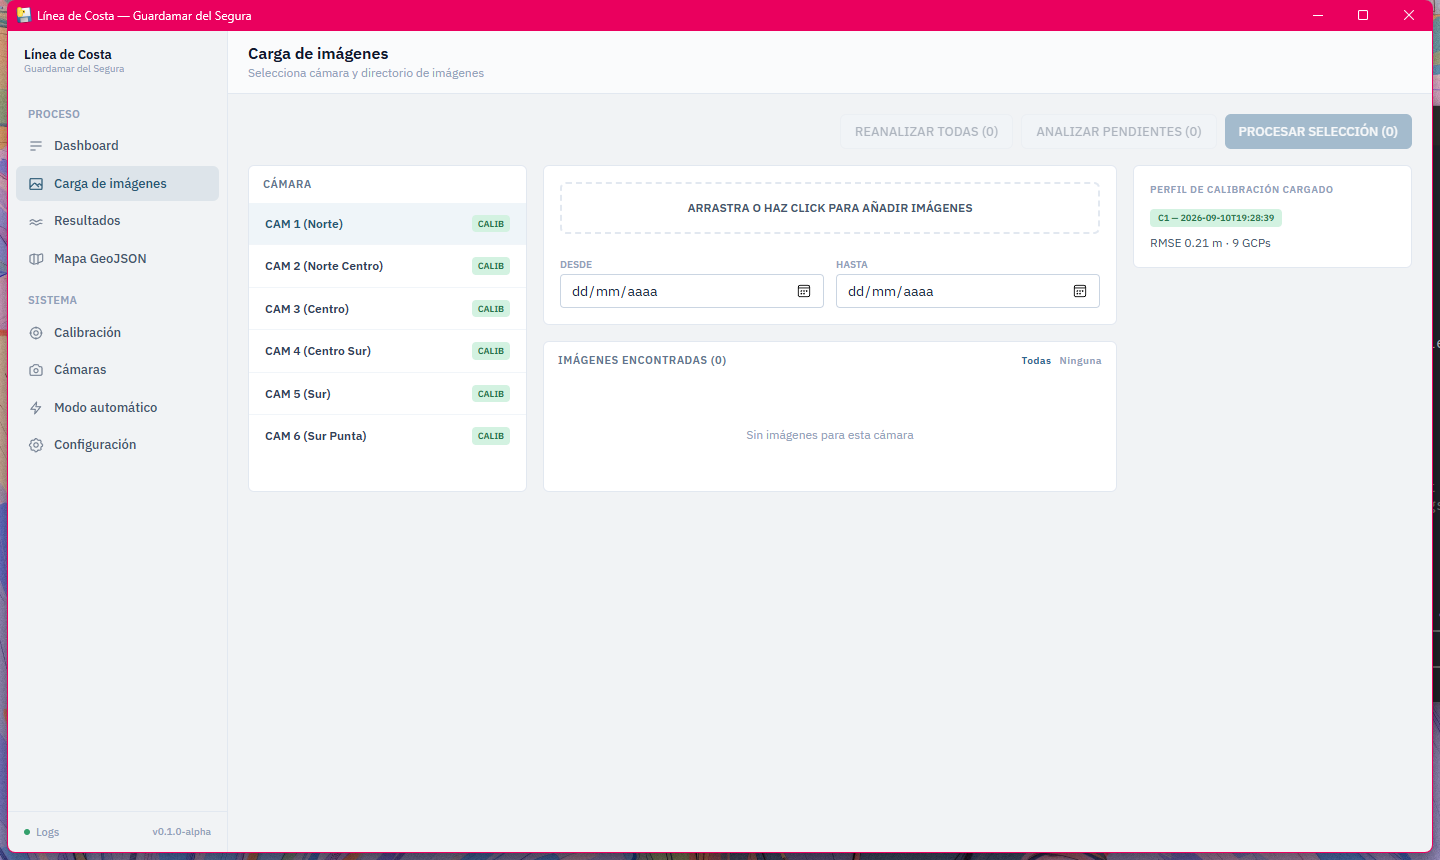
\includegraphics[width=0.95\textwidth]{screenshots/02_carga_imagenes.png}
\caption{Carga de imágenes — selector de cámara, zona de subida, filtro de fechas y perfil de calibración cargado.}
\end{figure}

\subsection{Resultados}

Pantalla principal de análisis: seleccionar cámara e imagen, pulsar \textit{Analizar imagen} y
revisar la línea de costa detectada y sus métricas.

\begin{figure}[H]
\centering
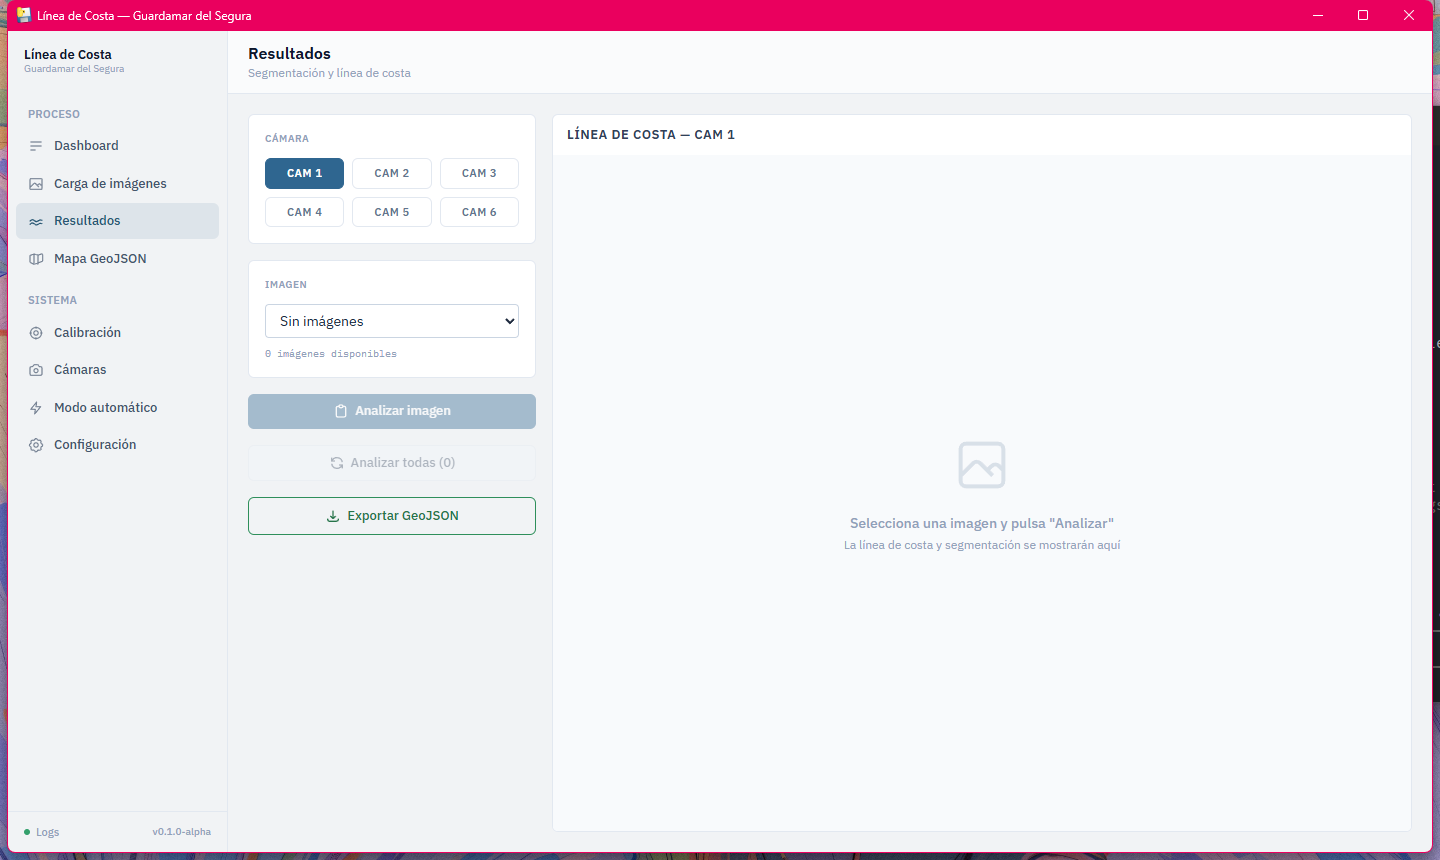
\includegraphics[width=0.95\textwidth]{screenshots/03_resultados.png}
\caption{Resultados — selector de cámara/imagen, panel de métricas y visor de la línea de costa.}
\end{figure}

\begin{itemize}[leftmargin=1.5em]
  \item \textbf{Flechas de navegación} (junto al título): pasan a la imagen anterior/siguiente de
        la lista. Si esa imagen \textbf{ya tiene} un resultado aceptado en el histórico, se
        muestra al instante, sin volver a analizar (\S\ref{sec:cache-por-imagen}); si nunca se
        analizó, se lanza un análisis real, igual que con el botón de siempre.
  \item \textbf{Analizar todas (N)}: analiza de golpe todas las imágenes de la cámara
        seleccionada, sin salir de esta pantalla — para ver la evolución completa sin ir a
        Carga de imágenes.
  \item \textbf{Panel de métricas}, de arriba a abajo:
    \begin{enumerate}
      \item \textbf{Confianza} — barra verde/ámbar/rojo.
      \item \textbf{Anchura de playa (transectos)} — un valor en metros por cada transecto
            marcado para esta cámara (\S\ref{sec:transectos}). Con la pantalla de Transectos
            oculta del menú a día de hoy, este apartado no aparece salvo que ya hubiera
            transectos marcados de antes.
      \item \textbf{Área seca (m\textsuperscript{2})} — se mantiene visible como referencia.
      \item \textbf{Puntos UTM} y \textbf{Timestamp}.
    \end{enumerate}
  \item \textbf{Editar línea manualmente} (botón junto al título, solo visible con un resultado
        aceptado): corrige a mano la línea cuando se equivoca — ver \S\ref{sec:edicion-manual}.
  \item \textbf{Exportar GeoJSON}: descarga el histórico completo de la cámara en un
        \texttt{.geojson} (EPSG:25830), listo para abrir en QGIS.
\end{itemize}

\subsubsection{Por qué las flechas no vuelven a analizar}
\label{sec:cache-por-imagen}

Cada análisis se guarda por nombre de fichero, tanto la imagen con la línea dibujada como el
resultado numérico. Navegar con las flechas a una imagen ya analizada consulta ese resultado
guardado en vez de relanzar el análisis — instantáneo, y no repite trabajo sobre fotos que no
han cambiado.

\subsubsection{Edición manual de la línea detectada}
\label{sec:edicion-manual}

Al pulsar \textit{Editar línea manualmente}, la imagen mostrada cambia de la visualización
(con la línea ya dibujada) a la \textbf{foto original}, con la línea detectada superpuesta como
puntos de control editables.

\begin{itemize}[leftmargin=1.5em]
  \item \textbf{Clic} sobre la imagen: añade un punto nuevo.
  \item \textbf{Arrastrar} un punto existente: lo mueve.
  \item \textbf{Doble clic} sobre un punto: lo borra.
  \item \textit{Guardar corrección}: guarda los puntos corregidos como dato de entrenamiento,
        en el mismo sitio que las polilíneas marcadas a mano en Entrenamiento
        (\S\ref{sec:entrenamiento}).
  \item \textit{Cancelar}: descarta los cambios sin guardar nada.
\end{itemize}

\subsection{Mapa GeoJSON}

Visualiza sobre un mapa real las líneas de costa detectadas de todas las cámaras, en EPSG:25830.

\subsection{Calibración}

Asistente de 7 pasos para establecer la correspondencia entre píxel de la imagen y coordenada
real en el terreno para cada cámara. No hace falta repetirlo salvo que la cámara se desplace de
forma notable (viento fuerte, limpieza brusca) o se añada una cámara nueva.

\begin{figure}[H]
\centering
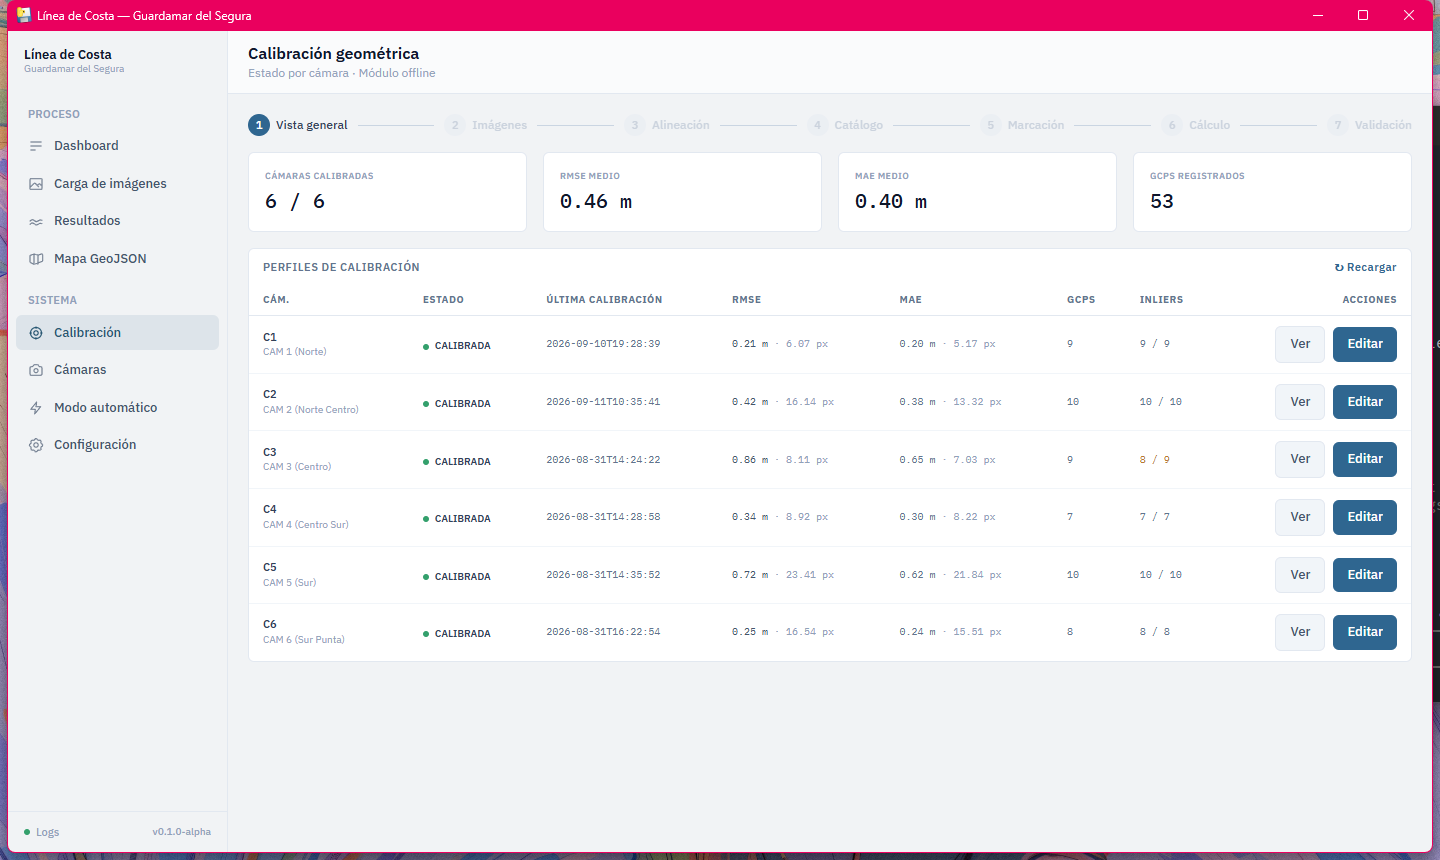
\includegraphics[width=0.95\textwidth]{screenshots/04_calibracion.png}
\caption{Calibración — vista general con el estado real de las 6 cámaras: RMSE, MAE, GCPs e inliers.}
\end{figure}

\subsection{Cámaras}

Configuración de hardware por cámara: lente, ROI (región de interés) y ubicación.

\begin{figure}[H]
\centering
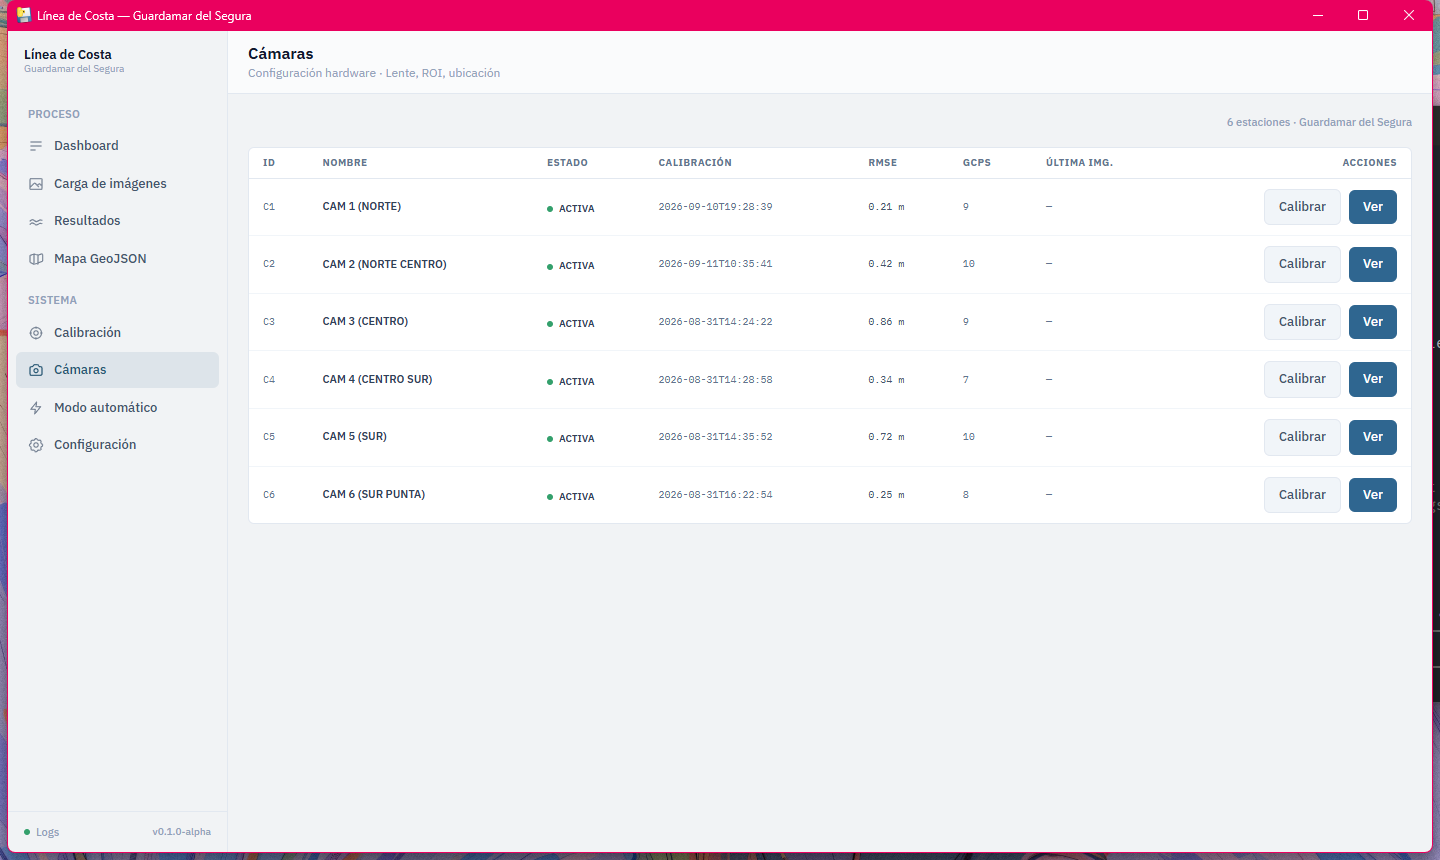
\includegraphics[width=0.95\textwidth]{screenshots/05_camaras.png}
\caption{Cámaras — estado de las 6 estaciones (RMSE, GCPs, fecha de calibración).}
\end{figure}

\subsection{Modo automático}

Automatiza de punta a punta, para un rango de fechas, lo que \textit{Carga de imágenes} y
\textit{Resultados} hacen a mano: descarga de imágenes, alineación y análisis. Requiere una
cámara ya calibrada.

\begin{figure}[H]
\centering
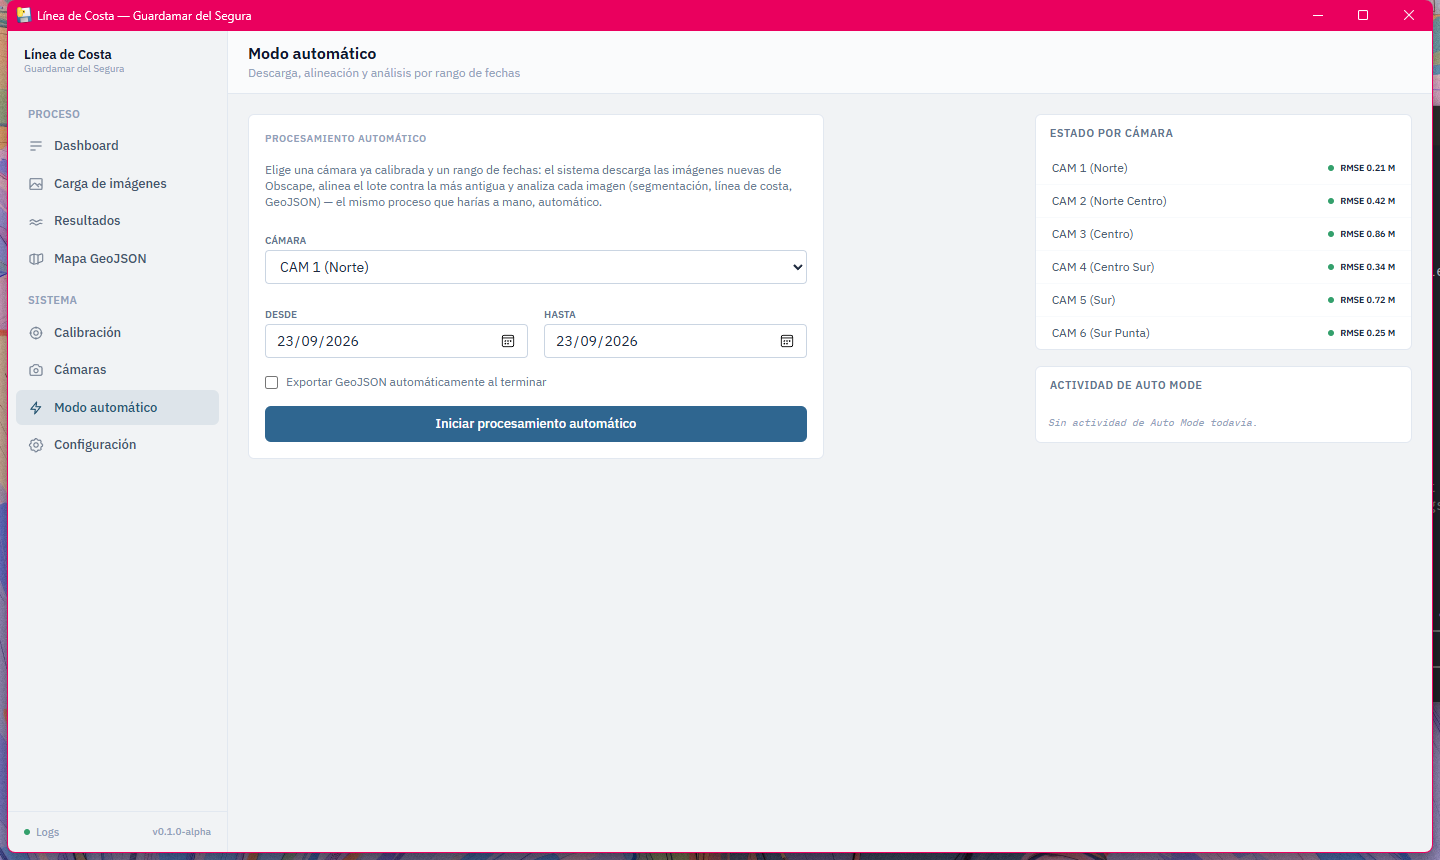
\includegraphics[width=0.95\textwidth]{screenshots/06_modo_automatico.png}
\caption{Modo automático — panel de procesamiento por rango de fechas y estado de RMSE por cámara.}
\end{figure}

\subsection{Configuración}

\begin{itemize}[leftmargin=1.5em]
  \item \textbf{Credenciales de Obscape}: usuario y clave de API para descargar imágenes — se
        guardan solo en este ordenador.
  \item \textbf{Ubicación de los datos}: rutas reales en disco de imágenes y calibración de este
        ordenador, con botón \textit{Copiar}.
  \item \textbf{Borrar imágenes y resultados}: acción destructiva e irreversible (requiere
        escribir \texttt{BORRAR} para confirmar) — elimina imágenes, varillas marcadas e
        histórico de las 6 cámaras. \textbf{La calibración no se toca.}
\end{itemize}

\begin{figure}[H]
\centering
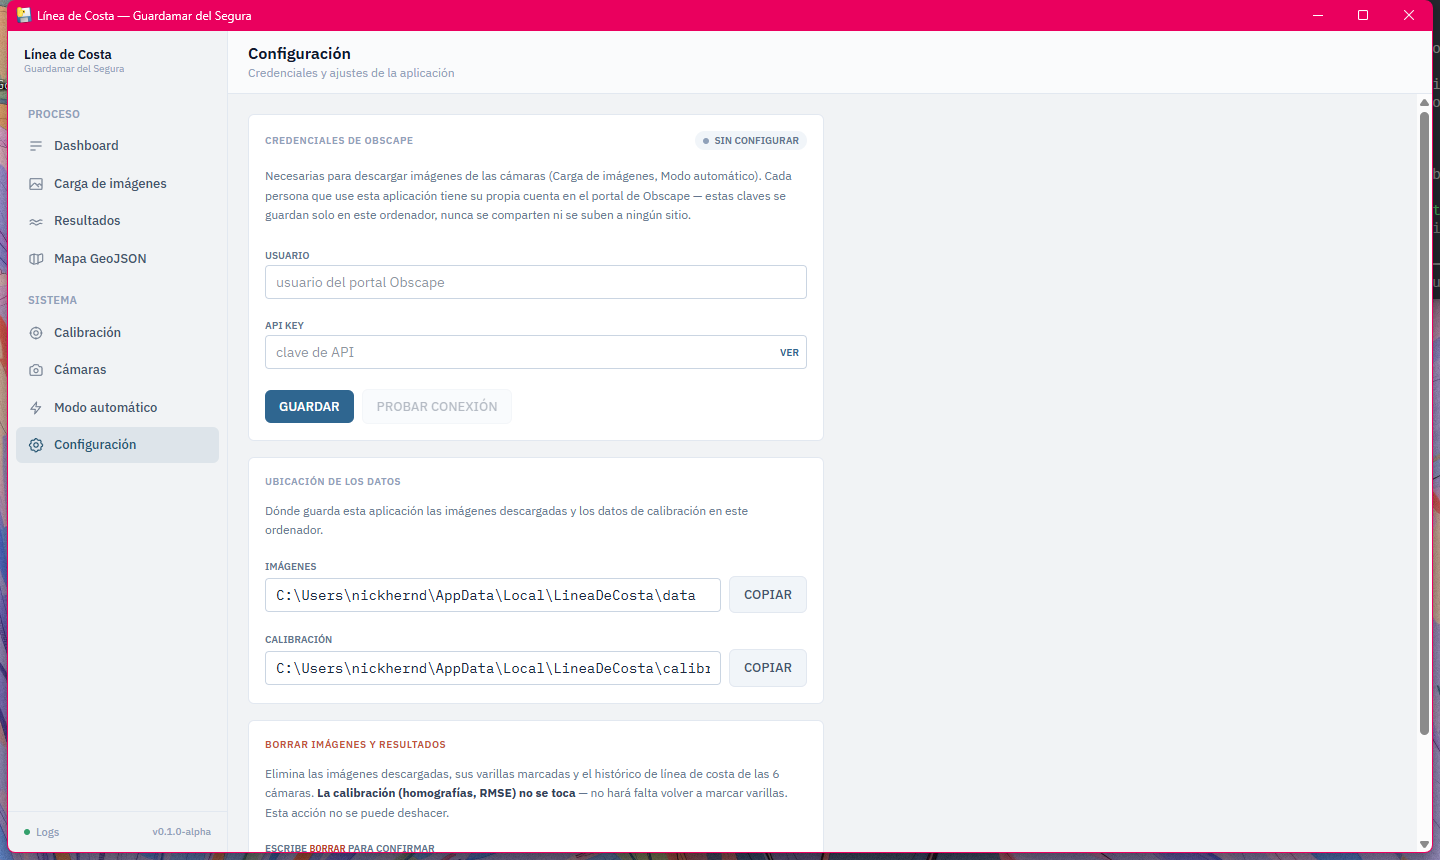
\includegraphics[width=0.95\textwidth]{screenshots/07_configuracion.png}
\caption{Configuración — credenciales de Obscape, ubicación de los datos y borrado de imágenes/resultados.}
\end{figure}

\section{Flujo de trabajo recomendado (día a día)}

\begin{enumerate}[leftmargin=1.5em, label=\textbf{\arabic*.}]
  \item \textit{Modo automático} (o \textit{Carga de imágenes} + \textit{Analizar pendientes})
        para procesar las imágenes nuevas de cada cámara ya calibrada.
  \item Revisar en \textit{Resultados} los rechazos y las confianzas bajas; si la línea
        detectada se equivoca de forma puntual, corregirla con \textit{Editar línea
        manualmente} en vez de descartar el análisis entero.
  \item Exportar el GeoJSON o el informe PDF cuando haga falta compartir resultados.
\end{enumerate}

\section{Funcionalidades en pausa}
\label{sec:en-pausa}

\begin{warnbox}[Sin botón de acceso en el menú a día de hoy (23/09/2026)]
Las dos pantallas de esta sección — \textit{Transectos} y \textit{Entrenamiento (temp.)} — no
tienen botón de acceso en el menú lateral en esta versión: se ocultaron a petición del usuario,
\textbf{no se eliminaron}. Siguen intactas y funcionando por dentro (un transecto ya marcado,
por ejemplo, se sigue calculando en cada análisis). Se documentan igualmente porque pueden
reactivarse en cualquier momento.
\end{warnbox}

\subsection{Transectos --- anchura de playa}
\label{sec:transectos}

Sustituye al área en m\textsuperscript{2} como indicador principal de evolución de la playa: un
punto de referencia \textbf{fijo} (p.\,ej. la valla de la duna) + la distancia hasta la línea de
costa detectada en cada análisis.

\begin{enumerate}[leftmargin=1.5em]
  \item Ir a \textbf{Transectos} en el menú lateral y elegir la cámara.
  \item Elegir una imagen de referencia (por defecto, la más reciente).
  \item \textbf{Clic} sobre la imagen para añadir un transecto — aparece en la lista de la
        izquierda con una etiqueta editable (p.\,ej. ``Valla duna norte'').
  \item \textit{Guardar cambios}.
\end{enumerate}

A partir de ahí, \textbf{cada análisis} de esa cámara calcula automáticamente la distancia de
cada transecto hasta la línea detectada y la muestra en el panel de métricas — no hace falta
volver a marcarlo. Un mismo transecto puede reutilizarse en todas las imágenes futuras de esa
cámara.

\subsection{Entrenamiento línea húmeda --- sección temporal}
\label{sec:entrenamiento}

\begin{warnbox}[Sección temporal]
Pensada para que el equipo de campo marque a mano dónde está la línea húmeda real en imágenes
reales, y así entrenar/ajustar la segmentación automática más adelante. No afecta a los
resultados de \textit{Resultados}.
\end{warnbox}

\begin{enumerate}[leftmargin=1.5em]
  \item Ir a \textbf{Entrenamiento (temp.)} en el menú lateral y elegir la cámara.
  \item Elegir una imagen de la lista desplegable (o subir una propia, ver más abajo).
  \item \textbf{Clic} sobre la imagen para ir añadiendo los puntos de la polilínea, en orden,
        siguiendo la línea húmeda real.
  \item \textit{Guardar polilínea}.
\end{enumerate}

\subsubsection{Zoom, lupa y ajuste fino}

\begin{itemize}[leftmargin=1.5em]
  \item \textbf{Completa / Doble zoom}: alterna entre la imagen ajustada al panel y el doble de
        tamaño (con scroll).
  \item \textbf{Zoom de la lupa} (×2 a ×15): recorte ampliado que sigue al cursor, para acertar
        el píxel exacto en fotos de varios miles de píxeles de ancho.
  \item \textbf{Clic sobre un punto ya puesto}: lo selecciona (se pone verde y más grande) sin
        moverlo.
  \item \textbf{Flechas del teclado}, con un punto seleccionado: lo desplazan 1~px (10~px con
        Mayús) — para el ajuste fino que el ratón no permite con precisión.
\end{itemize}

\subsubsection{Imágenes adicionales}

No hace falta que las imágenes a marcar sean las ya cargadas de la cámara: el botón \textit{Subir
imágenes adicionales} permite traer cualquier foto suelta solo para entrenamiento. Se pueden
eliminar de forma permanente con \textit{Eliminar esta imagen adicional}.

\subsubsection{Revisar y descartar antes de anotar}

El botón \textit{Descartar esta imagen} saca la imagen de la cola de anotación por defecto — es
un descarte \textbf{blando y reversible}: no borra el archivo. El checkbox \textit{Mostrar
descartadas (N)} las vuelve a mostrar, con la opción de \textit{Reincluir}.

\subsubsection{Exportar}

\textit{Exportar JSON (cámara)} descarga todas las polilíneas guardadas de la cámara actual en
un único fichero.

\end{document}
